\chapter{Proposal}

In this section we will set the goals and explain the design and an implementation of the Operating System, that is, the proposed solution to the requirement specifications and use cases presented in the previous chapter. This chapter is divided into two major sections:
\begin{enumerate}
	\item \textbf{Design} This part is about how the system is organized in an abstract way, that is, exposing the different parts of the system, their interactions as well as the design decisions and justification for the these parts.
	\item \textbf{Implementation} This part is the tangible part of the chapter: It shows the organization of the source code, code tree and source code snippets that are relevant for the proposal.
\end{enumerate}

\section{Design}

The design of the kernel is made using three different parts:
\begin{enumerate}
	\item \textbf{The Kernel Core}: The part of the kernel that deal with the hardware at very low level. This part mainly deals with the booting part as well as context switching and interrupts. This part is totally \textbf{architecture dependent}.
	\item \textbf{Kernel management}: Mainly drivers, this part is dedicated to memory management and management of the different hardware part of the Raspberry Pi.
	\item \textbf{Developer API}: This part is not directly needed by the kernel to properly work but it proposes an interface for the developer to use the kernel. It contains modules such as string management module, input/output module, thread module and graphical helper module.
\end{enumerate}


\begin{figure}[H]
\begin{center}
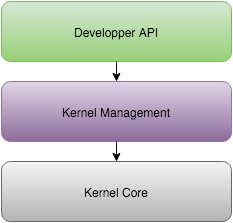
\includegraphics[width=0.5\textwidth]{includes/figures/chapter5_kernel_layers.png}  \\[0.5 cm]
\caption{Kernel layers}
\end{center}
\label{fig:chapter5_kernel_layers}
\end{figure}


\subsection{Kernel Core Layer}
As stated in the introduction, this part of the code is the heavily hardware dependent. It is the one dedicated to the low level interaction with the kernel and is overall dedicated to the CPU and partial interrupt management. Naturally, this part of the kernel is written in ARM assembly language.

This is the first part that has to be executed by the kernel once the Raspberry Pi bootstraping has finished and does in the early part:
\begin{enumerate}
	\item Set-up of the interrupt vector table.
	\item Set-up of the the Interrupt mode's, Fast Interrupt mode's and Supervisor mode's stack pointers.
	\item Jump to the very first bit of the C kernel code (Kernel management layer).
\end{enumerate}


It is also has two essential method that are dedicated to enabling and disabling interrupts.


This layer is indispensable for being able to boot code that is not programmed in assembly and also to handle interrupts in a later stage of the booting process, thanks to the set up of the interrupt vector table and setting up their stack pointers.



\subsection{Kernel Management Layer}
The kernel management is the part that contains different driver modules for the management of the different hardware part of the device. Each of these module have a different tasks that are separated by their main goals.

The diagram below shows the different modules present in this layer as well as their relations between each other. Some of them can be useful on their own (such as the malloc module or the queue module) and can therefore be used by the developer. Some other are only useful for a specific goal (such as the mailbox module, UART module or scheduler module).

\begin{figure}[H]
\begin{center}
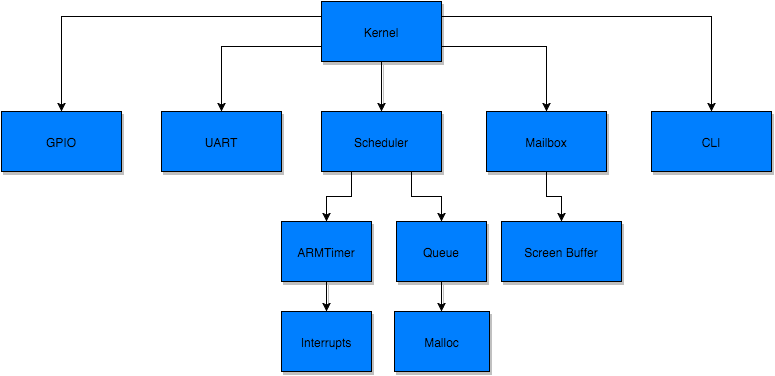
\includegraphics[width=1\textwidth]{includes/figures/chapter5_kernel_management_layer.png}  \\[0.5 cm]
\caption{Kernel Management Layers}
\end{center}
\label{fig:chapter5_kernel_management_layer}
\end{figure}


In the following section we will proceed to present each of these module by defining their goals and what the functions that are to be present.
 are
\subsubsection{Kernel module}
The kernel module is the conductor of the whole kernel. It does nothing by itself but instead manage all the required module for the correct initialization of the kernel and keeps sure that everything has been correctly initialized. After all the booting process, it finally runs the \textit{user program}, that is, the part of the code that is defined by the user. 

\begin{figure}[H]
\begin{center}
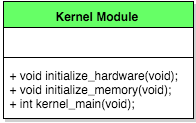
\includegraphics[width=0.4\textwidth]{includes/figures/chapter5_kernel_management_layer_kernel_UML.png}  \\
\caption{Kernel Management Layers - Kernel UML}
\end{center}
\label{fig:chapter5_kernel_management_layer_kernel_UML}
\end{figure}


As displayed on the UML graph, the kernel module has three functions:
\begin{itemize}
	\item \textbf{initialize\_hardware}: Aimed to initialize the UART as well as the frame-buffer for the HDMI outputs.
	\item \textbf{initialize\_memory}: Aimed to initialize the memory needed to use the malloc functions suite.
	\item \textbf{kernel\_main}: This is the function that is called after the kernel initilization (i.e. at the end of the Kernel core sequence). It calls the two previous functions.
\end{itemize}




\subsubsection{GPIO module}

\begin{figure}[H]
\begin{center}
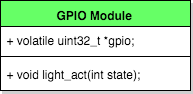
\includegraphics[width=0.4\textwidth]{includes/figures/chapter5_kernel_management_layer_GPIO_UML.png}  \\
\caption{Kernel Management Layers - GPIO UML}
\end{center}
\label{fig:chapter5_kernel_management_layer_GPIO_UML}
\end{figure}


As displayed on the UML graph, the GPIO module has only one functions: The light\_act function. This function is aimed to turn ON or OFF the ACT LED.
However, the important part of that module is that is had to define the constants and the variable required to manipulate said GPIO.




\subsubsection{UART module}

\begin{figure}[H]
\begin{center}
\includegraphics[width=0.4\textwidth]{includes/figures/chapter5_kernel_management_layer_UART_UML.png}  \\
\caption{Kernel Management Layers - UART UML}
\end{center}
\label{fig:chapter5_kernel_management_layer_UART_UML}
\end{figure}


As displayed on the UML graph, the kernel module has five functions:
\begin{itemize}
	\item \textbf{uart\_write\_char}: Aimed to send a byte to the UART hardware. It is typically to write a character.
	\item \textbf{uart\_write}: Aimed to send an array of byte to the UART hardware. It is typically to write a string by recursively called \textit{uart\_write\_char}
	\item \textbf{uart\_read}: Aimed to receive a byte from the UART hardware.
	\item \textbf{uart\_init}: Realize a sequence of instruction aimed to set up the UART communication. It is it to set up the BAUD rate, storing policy, etc.
	\item \textbf{uart\_get\_input\_buffer}: Empty the UART buffer and returns its content to the caller.
\end{itemize}





\subsubsection{Scheduler module}

\begin{figure}[H]
\begin{center}
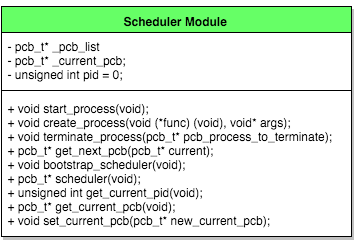
\includegraphics[width=0.7\textwidth]{includes/figures/chapter5_kernel_management_layer_scheduler_UML.png}  \\
\caption{Kernel Management Layers - Scheduler UML}
\end{center}
\label{fig:chapter5_kernel_management_layer_scheduler_UML}
\end{figure}


This module is the biggest and the most complex module in term of code and covers many different features as it handle everything from the context structure declaration up to the scheduler algorithm and the context switching. An important element that is the pillar of this module is the \textit{pcb\_list}. This is a queue (see the queue module) that contains the list of the ready-to-start and started processes. Let's detail all the functions and what their purpose is:
\begin{itemize}
	\item \textbf{create\_process}: This function is in charge of creating a process, that is, creating its metaphor (a PCB \footnote{Process Control Block}), dedicating dynamically its stack memory (see the malloc module), setting up its state and finally inserting the created PCB to the \textit{pcb\_list}.
	\item \textbf{start\_process}: As indicated by its name, it starts a previously created process. When a process is created, it is allocated in memory and the metaphor is initialized with the adequate initial values. Start\_process takes a PCB as parameter and start the process that the PCB refers to.
	\item \textbf{terminate\_process}: This function takes also a PCB as parameter. It terminates the process that the PCB refers to, that is, cleaning the memory related to process (its stack and the PCB structure itself).
	\item \textbf{get\_next\_pcb}: Returns the PCB of the next executable process (i.e. newly created or paused due to a context switch). This is the function mainly used for the Round-Robin scheduling algorithm.
	\item \textbf{scheduler}: This function is to be called to get the next PCB to schedule. In the current design, it simply calls \textit{get\_next\_pcb}, but it is aimed to be able to call any other function depending on the algorithm that the user wants to develop.
	\item \textbf{get\_current\_pid}: System function that a process can run to get its PID\footnote{Process ID, typically an integer that uniquely defines a process}.
	\item \textbf{get\_current\_pcb}: Function that returns the whole PCB of the process currently scheduled to the caller.
	\item \textbf{set\_current\_pcb}: Set the current PCB, that is, the PCB that will be scheduled next.
	\item \textbf{bootstrap\_scheduler}: System function that can be called in order to start the scheduling process, that is: enable the interrupt, set up the ARM timer and ARM timer interrupt, start the first process in the PCB list. This function has to be called only once and assumes that at least one process ready to be scheduled has been inserted into the PCB list.
	\item \textbf{set\_current\_pcb}: Set the current PCB, that is, the PCB that will be scheduled next.
\end{itemize}



\subsubsection{ARMTimer module}


\begin{figure}[H]
\begin{center}
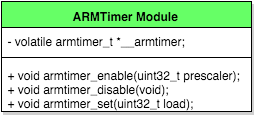
\includegraphics[width=0.5\textwidth]{includes/figures/chapter5_kernel_management_layer_ARMTimer_UML.png}  \\
\caption{Kernel Management Layers - ARMTimer UML}
\end{center}
\label{fig:chapter5_kernel_management_layer_ARMTimer_UML}
\end{figure}


This module is a simple one that is aimed to set up the ARMTimer as well as its interrupt. It only contains three functions:
\begin{itemize}
	\item \textbf{armtimer\_enable}: Enable the timer: Enable the interrupt and set its pre-scaler, that is the amount of cycle that have to be reach to decrement the counter of the timer by one. Once the timer reaches \textit{zero}, an interrupt is triggered. The starting value of the counter is set by the function \textit{armtimer\_set}.
	\item \textbf{armtimer\_disable}: Disable the timer interrupts.
	\item \textbf{armtimer\_set}: Set the timer initial value to the argument that is passed to the function. 
\end{itemize}




\subsubsection{Interrupts module}

\begin{figure}[H]
\begin{center}
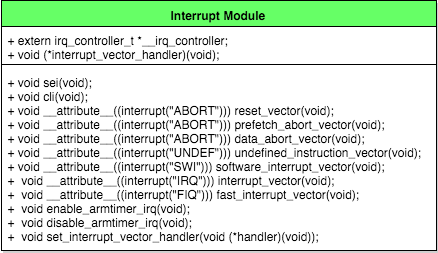
\includegraphics[width=0.7\textwidth]{includes/figures/chapter5_kernel_management_layer_interrupts_UML.png}  \\[0.5 cm]
\caption{Kernel Management Layers - Interrupts UML}
\end{center}
\label{fig:chapter5_kernel_management_layer_interrupts_UML}
\end{figure}

As its name suggests, this class is where the interrupt handlings are made. It has one function for each interrupt but several or them are actually not used in this kernel but are needed to be defined nontheless. It also contains functions that can enable or disable the interrupts handling. All these function are explained below:

\begin{itemize}
	\item \textbf{sei}: Enable the interrupt handling. That is, if an interrupt is triggered, the kernel will execute the appropriate handler.
	\item \textbf{cli}: Disable the interrupt handling. That is, if an interrupt is triggered, no handler will be executed. This functions mainly used for critical sections (i.e.: Sections that shouldn't be interrupted).
	\item \textbf{reset\_vector}: Handler that is triggered during the reset flavour of the \textit{ABORT} interrupt.
	\item \textbf{prefetch\_abort\_vector}: Handler that is triggered during the prefect abort flavour of the \textit{ABORT} interrupt. This handler is not implemented.
	\item \textbf{data\_abort}: Handler that is triggered during the data abort flavour of the \textit{ABORT} interrupt. This interrupt is triggered when having a data fault in the kernel. The interrupt shows a debug message in order to pinpoint the address of the instruction that triggered the data abort interrupt and then cause the kernel to hang.
	\item \textbf{undefined\_instruction\_vector}: Handler that is triggered during an \textit{UNDEF} interrupt. This handler is not implemented.
	\item \textbf{software\_interrupt\_vector}: Handler that is triggered during an \textit{SWI} interrupt (software interrupt). This handler is not implemented as no function trigger software interrupts are implemented.
	\item \textbf{interrupt\_vector}: Handler that is triggered during an \textit{IRQ} interrupt (hardware interrupts). This the interrupt in charge of performing the tasks to be performed at each interrupt generated by the ARMTimer. It is design to read the input received on the UART, and then perform the scheduling and context switch to the next process.
	\item \textbf{fast\_interupt\_vector}: Handler that is triggered during an \textit{FIQ} interrupt (fast interrupt). This handler is not implemented.
	\item \textbf{enable\_armtimer\_irq}: Enable specifically the arm interrupts.
	\item \textbf{disable\_armtimer\_irq}: Disable specifically the arm interrupts.
\end{itemize}


\subsubsection{Queue module}


\begin{figure}[H]
\begin{center}
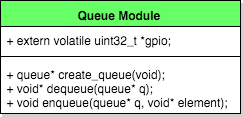
\includegraphics[width=0.5\textwidth]{includes/figures/chapter5_kernel_management_layer_queue_UML.png}  \\
\caption{Kernel Management Layers - Queue UML}
\end{center}
\label{fig:chapter5_kernel_management_layer_queue_UML}
\end{figure}

This module basically defines and handle the queue data structure. A queue is a linear data structure. This data structure present a head and a tail with an element that linked to the next (if any) by storing its value. A queue is always processed from the head to the tail: The next element to be dequeued is the element on the head and when adding an element, it becomes the next tail, this makes it a FIFO\footnote{First-In First-Out} data structure.
It only contains three functions:
\begin{itemize}
	\item \textbf{create\_queue}: It simply create the queue data structure that can then be used with the \textit{dequeue} and \textit{enqueue} functions.
	\item \textbf{dequeue}: As aformentioned, deleting the head of the queue and returning the element in contains. The element that was next to the head is now the new head.
	\item \textbf{enqueue}: This function add an element to the queue and place it right after the tail of the queue, becoming the new tail of the queue.
\end{itemize}


\subsubsection{Malloc module}


\begin{figure}[H]
\begin{center}
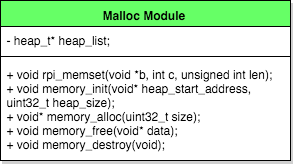
\includegraphics[width=0.6\textwidth]{includes/figures/chapter5_kernel_management_layer_malloc_UML.png}  \\
\caption{Kernel Management Layers - Malloc UML}
\end{center}
\label{fig:chapter5_kernel_management_layer_malloc_UML}
\end{figure}

This module is aimed to provide support to dynamics memory allocation, that is, allocate memory of a dynamic size at run time instead of using the compiler to allocate memory at compile time. This module is specially useful when creating process for the PCB allocation as well at the stack allocation. The specifics of this module are explained in the dedicated part implementation section.
Many function are purposely named at their UNIX counterpart as they mimic their behaviour. The list of the function of this module is described hereafter:
\begin{itemize}
	\item \textbf{rpi\_memset}: It has the same behaviour that you'd expect from the UNIX's \textit{memset}, that is, given a memory address, a value and a length, the function fills the memory address by the value provided and for a number of bytes provided by the length.
	\item \textbf{memory\_init}: This function is needed to be called first before being able to use \textit{memory\_alloc}. Given a memory segment (an address and a length) that will be dedicated to dynamic memory, it creates a \textit{queue} where each element represents a dynamic memory allocation (or a freed one that my be used for another memory allocation).
	\item \textbf{memory\_alloc}: This the kernel's version of UNIX's \textit{malloc}. Given a length in byte, it returns the starting address of a memory segment of the length provided to the function.
	\item \textbf{memory\_free}: Free a memory segment so as to be useful for another memory allocation later in time.
	\item \textbf{memory\_destroy}: This is the reverse of the function \textit{memory\_init}: It frees all the memory segment allocated in the dynamic memory segment and then destroys said memory segment.
\end{itemize}


\subsubsection{Mailbox module}


\begin{figure}[H]
\begin{center}
\includegraphics[width=0.6\textwidth]{includes/figures/chapter5_kernel_management_layer_mailbox_UML.png}  \\
\caption{Kernel Management Layers - Mailbox UML}
\end{center}
\label{fig:chapter5_kernel_management_layer_mailbox_UML}
\end{figure}

The Mailbox module creates the data structure to manipulate the Raspberry's mailbox with ease as well as method that are able to write and read the mailbox according to the board's specifications. It contains only two functions:
\begin{itemize}
	\item \textbf{mailbox\_write}: Given a channel number and an octet of data, sends the provided data to the mailbox on the given channel. 
	\item \textbf{mailbox\_read}: Given a channel, read data from a channel and returns it if any.
\end{itemize}


\subsection{CLI module}
\begin{figure}[H]
\begin{center}
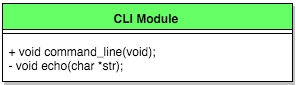
\includegraphics[width=0.6\textwidth]{includes/figures/chapter5_kernel_management_layer_cli_UML.png}  \\
\caption{Kernel Management Layers - CLI UML}
\end{center}
\label{fig:chapter5_kernel_management_layer_mailbox_UML}
\end{figure}

The CLI is the module made for user interactions. The module, as its name suggests, is designed to be able to interpret user's input and execute different commands. Here, only the part made to retrieve the inputs from the user, be able to get the function to run (first word) and pass the argument to the function (is the function is recognized, the arguments is what is directly placed after the function). For now, only the \textit{echo} function is being implemented.
\begin{itemize}
	\item \textbf{command\_line}: Spawn the CLI. When the function is run, is shows a command prompt and asks for the user to enter a command. 
	\item \textbf{echo}: Function available for the CLI. It simply mirrors to the serial interface what has been passed as argument.
\end{itemize}

\pagebreak



\subsection{Developer API Layer}
The developer API layer is the layer that is a lot higher level than the previous Kernel Management Layer. The four modules included into this layer are not considered as the necessary parts of the kernel to work but are nonetheless handy while developing other module, debugging or creating new interactions. As a result, these modules are lot more hardware-independent (unlike the ones from the Kernel Management Layer). This part also contains modules that were developed in a later stage of the project. This sections is here to present these modules.

Although these modules are a lot less interdependent, some of them still depend on others. This is the case of the Screen Text module that depends on the character module and the Standard Input/Output that depends on the Strings module.
Below is a presentation of these four modules: 




\subsubsection{Character module}

\begin{figure}[H]
\begin{center}
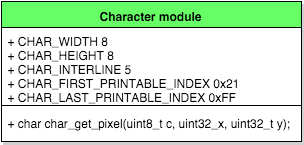
\includegraphics[width=0.6\textwidth]{includes/figures/chapter5_developper_api_layer_char_UML.png}  \\
\caption{Developper API Layer - Character UML}
\end{center}
\label{fig:chapter5_developper_api_layer_char_UML}
\end{figure}

This module is very simple yet very handy. It helps the Screen Text module to print character of the HDMI monitor without having to worry about the type face and the pixels to be printed. The only function of this module, \textit{char\_get\_pixel}, is able to return given a character, a x and y position within the dimensions of the font, the pixel color of the character.




\subsubsection{Screen Text module}

\begin{figure}[H]
\begin{center}
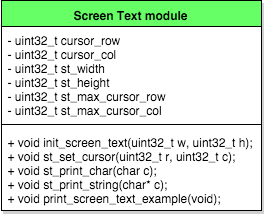
\includegraphics[width=0.6\textwidth]{includes/figures/chapter5_developper_api_layer_st_UML.png}  \\
\caption{Developper API Layer - Screen Text UML}
\end{center}
\label{fig:chapter5_developper_api_layer_st_UML}
\end{figure}

This module is in charge of displaying character on the HDMI output. It keeps track of the pointer and handles jump line. It is directly dependent on the \textit{Character module}. The function that it comprises are the following:
\begin{itemize}
	\item \textbf{init\_screen\_text}: Initializes the screen text (i.e. set the applicable width and height in pixel as well as setting the cursor boundaries).
	\item \textbf{st\_set\_cursor}: Sets the cursor to a given line and column.
	\item \textbf{st\_print\_char}: Prints a character on the current cursor position and update the cursor's position. This is the part that depends on the Character module.
	\item \textbf{st\_print\_string}: Recursively call the \textit{st\_print\_char} character so as to be able to print a string.
	\item \textbf{print\_screen\_text\_example}: Example of how to use the module. Use for presentation or testing purposes.
\end{itemize}




\subsubsection{Strings module}

\begin{figure}[H]
\begin{center}
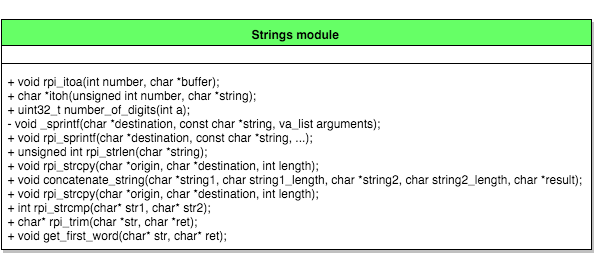
\includegraphics[width=1\textwidth]{includes/figures/chapter5_developper_api_layer_strings_UML.png}  \\
\caption{Developper API Layer - Strings UML}
\end{center}
\label{fig:chapter5_developper_api_layer_strings_UML}
\end{figure}

This module is similar to UNIX's \textit{string} library. This module is capable of handling several strings manipulations. The functions that it implements are described below:
\begin{itemize}
	\item \textbf{number\_of\_digits}: Given an integer, it returns the number of character needed to print said integer.
	\item \textbf{rpi\_itoa}: Integer to string function - Given a number and a character pointer, write the string representation of the number into the character pointer.
	\item \textbf{itoh}: Integer to hexadecimal function - Given a number and a character pointer, write the hexadecimal representation of the number into the character pointer.
	\item \textbf{\_sprintf}: Internal function of the \textit{sprintf} function described below. Given a character pointer (aimed to be the destination), a string with variable place holders and a list of arguments, writes into the destination the formatted string in relation to the arguments.
	\item \textbf{sprintf}: Function consuming the \textit{\_sprintf}. It takes care of the variable number of arguments handling before passing them the \textit{\_sprintf}.
	\item \textbf{rpi\_strlen}: Given a null-ended string, returns its length (i.e.: Number of character until meeting the \textit{null} character).
	\item \textbf{rpi\_strcpy}: Given an origin and a destination char pointer as well as a length, copy the \textit{length} first characters of the origin to the destination.
	\item \textbf{concatenate\_string}: Given a first string, its length, a second string, its length and a destination string (that is assumed to have a length bigger than the sum of the two previous strings), writes the concatenation of the two strings to the destination.
    \item\textbf{rpi\_strcmp:} Returns \textit{EQUAL\_STRINGS} if two strings are equals, \textit{DIFFERENT\_STRINGS} else.
    \item\textbf{rpi\_trim:} Copies the content of the input strings into a destination string removing the leading and trailing spaces.
    \item\textbf{get\_first\_word:} Returns the first word found on the input string into the destination string.
\end{itemize}





\subsubsection{Standard Input/Output}

\begin{figure}[H]
\begin{center}
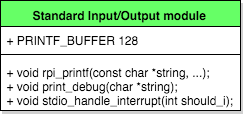
\includegraphics[width=0.5\textwidth]{includes/figures/chapter5_developper_api_layer_stdio_UML.png}  \\
\caption{Developper API Layer - Strings UML}
\end{center}
\label{fig:chapter5_developper_api_layer_stdio_UML}
\end{figure}

The Sandard Input/Output module is in charge of providing some standard API for printing on the serial port. It has three functions:
\begin{itemize}
	\item \textbf{rpi\_printf}: Homologous function of the widely known UNIX \textit{printf} function adapted for this kernel. It internally uses \textit{sprintf} to format the string and then prints said string on the serial port using the UART module.
	\item \textbf{print\_debug}: Function that prints a given string onto the serial port if and only if the kernel has been compiled with the \textit{DEBUG} flag.
	\item \textbf{stdio\_handle\_interrupt}: It is important that this functions of this module are not interrupted (via any kind of interrupt) while they are being executed. This is due to the interaction with the serial port as well as the data that it contains that might be switched be replaced by another thread's argument. Not taking care of the interrupt while using either of the previously mentioned method can trigger a data abort interruption.
\end{itemize}


\pagebreak




\section{Implementation}
This part is aimed to present the tangible part of the project, that is, the source code. It also presents the hierarchy of the project as well as presenting the implementation of some components that are deemed necessary to be explained.

\subsection{Source code tree}
The source code tree is the organization of the source code, that is the folder organization of the code, how the code is structured, and explaining the reasoning being such structure.

Below is the directory tree of the source code with on the right-hand side of the directory or file, a description of its purpose:

\begin{figure}[H]
\dirtree{%
.1 /.
.2 Makefile \hspace{1.1cm} \ldots{}
             \begin{minipage}[t]{10cm}
                Makefile of the whole project{.} An extended description thereof can be found below{.}
            \end{minipage}.
.2 boot/ \hspace{1.65cm} \ldots{}
             \begin{minipage}[t]{10cm}
                Contains all the file that need to be copied the SD card{.}
            \end{minipage}.
.2 include/ \hspace{1.1cm} \ldots{}
             \begin{minipage}[t]{10cm}
                Contains the header files{.}
            \end{minipage}.
.3 data/ \hspace{1.15cm} \ldots{}
             \begin{minipage}[t]{10cm}
                Contains additional data such as pictures or fonts{.}
            \end{minipage}.
.2 linker\_map.s \hspace{0.35cm} \ldots{}
             \begin{minipage}[t]{10cm}
                Linker data for the compilation{.}
            \end{minipage}.
.2 memory\_map.d \hspace{0.35cm} \ldots{}
             \begin{minipage}[t]{10cm}
                Internal memory organization of the executable{.}
            \end{minipage}.
.2 obj/ \hspace{1.85cm} \ldots{}
             \begin{minipage}[t]{10cm}
                Temporary storage of the {.}o files{.}
            \end{minipage}.
.2 src/ \hspace{1.85cm} \ldots{}
             \begin{minipage}[t]{10cm}
                Folder containing the {.}c files{.}
            \end{minipage}.
.3 tests/ \hspace{1cm} \ldots{}
             \begin{minipage}[t]{10cm}
                Folder containing the unitary and functional tests{.} An extended description can be found in the Testing section{.}
            \end{minipage}.
.3 Makefile .
.3 obj/ .
.3 run\_test.sh \hspace{0.05cm} \ldots{}
             \begin{minipage}[t]{10cm}
                Bash script that runs all the tests at once{.}
            \end{minipage}.
.3 src/ \hspace{1.35cm} \ldots{}
             \begin{minipage}[t]{10cm}
                {.}c files of the tests{.}
            \end{minipage}.
}
\caption{Source tree}
\end{figure}


\subsection{Makefile}
The Makefile is the special text file format that allows the mapping of rules to commands as well as command dependency (i.e. a command needs to have its dependencies fulfilled before said command can be run). This is the method that has been chosen for this project for the compilation of the kernel as well as some handy functions that are useful for the user. The more interesting commands and what is their effect while using the Makefile are presented below:
\begin{itemize}
	\item \texttt{make all}: Same as doing both \texttt{make bootfiles} and \texttt{make gcc}\cite{osdev_rpi_bare_bone}
	\item \texttt{make bootfiles}: Download using \textit{curl} the latest boot-files from the official rapsberry-pi repository and store these files into the \textbf{./boot} folder.
	\item \texttt{make gcc}: Compile the project's kernel and place it into the \textbf{./boot} folder.
	\item \texttt{make deploy}: Copy the \textit{kernel.img} file previously compiled with \texttt{make gcc} and place it into the SD Card. It then prints both SHA values to be sure that the kernel has been correctly copied. Please note that this command may vary from one machine to another and might need customization.
	\item \texttt{make connect}: Connect to the raspberry-pi using screen and the baud-rate used in the kernel. It assume that \textit{screen} is installed on the system. Please note that as well as the previous command, the command might need to be adjusted on the machine.
\end{itemize}


\subsection{Booting process of the kernel}
While starting the Raspberry Pi, its own boot-loader is executed, this process has been explained on subsection \ref{chapter2_booting_process} - Booting Process. In this section we are going to talk about the kernel's boot-process, that is, the initialisation of our kernel once the Raspberry Pi is executing the custom code (i.e.: the one we compiled).

Below is a sequence diagram showing the booting process of the kernel from the moment the Raspberry Pi starts executing the code of the kernel up to the moment it executes the main program (that is, the user's code).


\begin{figure}[H]
\begin{center}
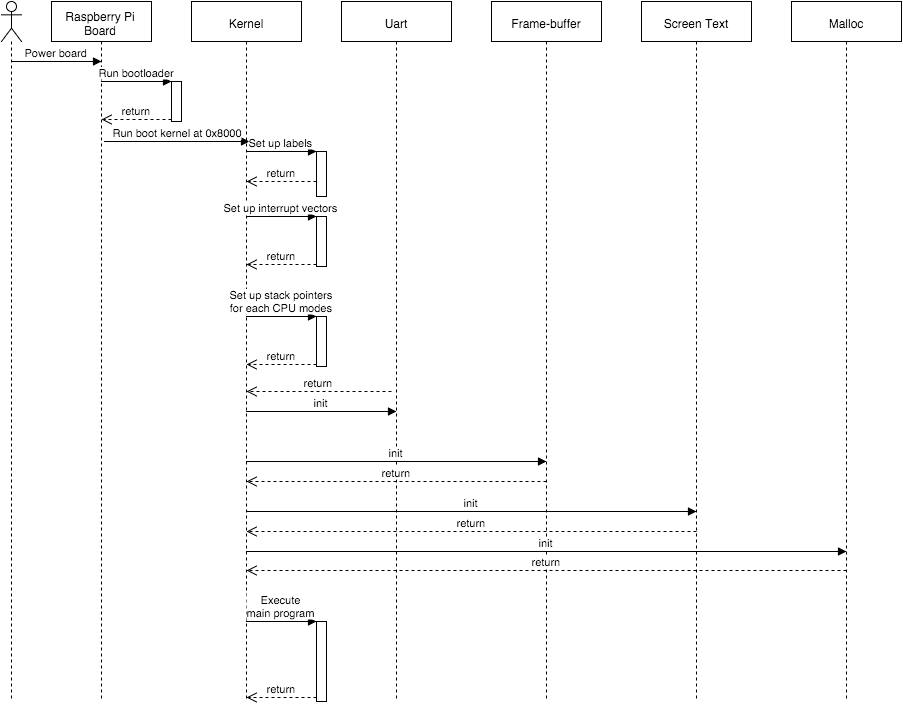
\includegraphics[width=1\textwidth]{includes/figures/chapter5_kernel_booting_sequence.png}  \\
\caption{Kernel Booting Sequence - Sequence Diagram}
\end{center}
\label{fig:chapter5_kernel_booting_sequence}
\end{figure}





\subsection{Dynamic memory allocation}
As aforementioned, dynamic memory allocation is something that is not only expected to be handled by the Operating System but also needed for its functioning. It allow the allocation of memory segments by a program without prior knowledge of how many bytes have to be allocated and how many memory segments will be allocated during the life cycle of the operating system execution. This sections explains how this has been implemented in this project.

Let's first begin by introducing the memory structure that has been chosen for the memory allocation. The heap is a single-linked queue with the following data structure:

\lstset{language=C}
\begin{figure}[H]
\begin{minipage}{\linewidth}
\begin{lstlisting}[frame=single]
struct heap_t
{
    char   size;          // Size of the allocated memory chunk
    char   allocated;     // Is it currently allocated or has it been freed?
    struct heap_t *next;  // Next element in the single-linked queue
};
\end{lstlisting}
\end{minipage}
\caption{Heap data structure}
\end{figure}

Each of the components of these elements is critical for the right functioning of heap. Let's details them:
\begin{itemize}
	\item \textbf{size}: This is the size of the chunk. It helps a lot in conjunction to the variable \textit{allocated} as it allow later memory allocation when the size is inferior than or equal to a previous dynamic memory chunk that has been freed.
	\item \textbf{allocated}: Gives information on whether or not the current chunk is being used (value \textit{ALLOCATED}) or freed (value \textit{UNALLOCATED}) and therefore eligible for a subsequent allocating on this particular memory chunk.
	\item \textbf{next}: The pointer to the next \textit{heap\_t} element in the heap.
\end{itemize}

A representation of the heap memory can be found bellow. It showcases the aforementioned data structure and the writable memory.

\begin{figure}[H]
\begin{center}
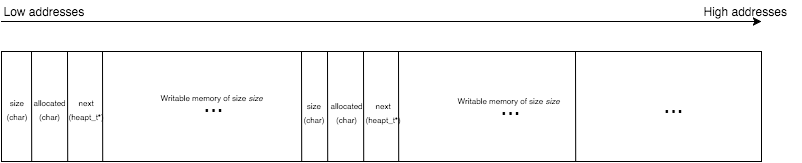
\includegraphics[width=1\textwidth]{includes/figures/chapter5_heap_representation.png}  \\
\caption{Representation of the heap}
\end{center}
\label{fig:chapter5_heap_representation}
\end{figure}

During the introduction to the malloc module, we presented the function \textit{memory\_init}. This function is the one readying the heap of the kernel for memory allocation, that is, it stores the starting value of the heap and write 0 for as long as the length allow us to (this is to ensure no garbage values in the memory heap).

The \textit{memory\_alloc} function is the one that does all the management on whether or not a memory can be allocated on a given memory chunk. It's pseudo-code is presented below.

\lstset{language=C}
\begin{figure}[H]
\begin{minipage}{\linewidth}
\begin{lstlisting}[frame=single]
void* memory_alloc(uint32_t size) {
    h = get_heap_start()    // Memory address of the elected chunk
    if (h != 0) do // First memory allocation
        while true do
            if h > heap_limit OR ((h == NULL OR h->allocated == UNALLOCATED) do
                break
            else
                h = h->next
            done
        done
    done
    
    if h > heap_limit do // Heap full
        return NULL 
    done
    
    // We have a valid chunk
    h->size = size;
    h->allocated = allocated;
    write_zeros_on_writable_memory(h)
    
    if h->next == NULL do
        h->next = h + sizeof(heap_t) + size
    done
    
    
    return h + sizeof(heap_t)   // Return the address of the writable memory
}
\end{lstlisting}
\end{minipage}
\caption{Heap data structure}
\end{figure}


What the function does is basically to iterate through the linked list and find either an eligible chunk or reach the end of the heap by checking the \textit{heap\_limit} variable. In case of failure, the function returns \textit{NULL}, and in case of success, the function returns the address of the writable memory.

In terms of complexity, we are iterating through the whole linked list. So the time complexity of the algorithm is $O(n)$.




\subsection{Context Switching}
Context switching is one of the key parts of this kernel and of an Operating System in general as one is expected to implement multi-tasking. In order to understand the implementation, let's first introduce how context are stored by presenting the data structure thereof. A snippet of the kernel code can be found on figure \ref{fig:chapter5_context_pcb_data_structure}.

As we can see, two figure are set. The first one is the context structure, it is aimed to store the information of a process at a given time. It store the stack pointer as well as the link pointer. Also, it store the original address of the stack pointer. This is needed in order to be able to destroy the memory segment of the stack pointer once we can to destroy the whole process. We can then find the structure of the Process Control Block, that is, the information related to the process in general (ID, its current state, the function that it runs, etc.).

\lstset{language=C}
\begin{figure}[H]
\begin{minipage}{\linewidth}
\begin{lstlisting}[frame=single]
typedef enum {NEW, READY, RUNNING, WAITING, TERMINATED} State;

// Definition of a context
typedef struct {
    unsigned int* sp_origin; // Origin of the stack pointer,
                             // needed for context destruction
    unsigned int* sp;        // Stack pointer
    unsigned int* lr;        // Link register
} context_t;


// Definition of the process control block
struct pcb_t {
    unsigned int  pid;                 // Process indentifier
    State         state;               // State of the process (new, ready, etc.)
    unsigned int  priority;            //The lower the more priority, linux convention
    void          (*function) (void);  // Function that the process will run
    void*         arguments;           // Arguments to be passed to the function
    context_t     context;
    struct pcb_t  *next;               // Next PCB in the single list
};
\end{lstlisting}
\end{minipage}
\caption{Presentation of Context and PCB data structure}
\label{fig:chapter5_context_pcb_data_structure}
\end{figure}


The part of the code dedicated to performing that context switch is present inside the function \textit{interrupt\_vector} inside the \textit{interrupts.c} file. Most of the code prior to that context switch is dedicated to choosing the next PCB to and therefor the next process that will be switched. As stated by the requirement specification, the policy used for the scheduling is Round Robin without priority, that is, the PCB are chosen with the order they have been added to the PCB list and are all allocated a fixed amount of time.

\begin{figure}[H]
\begin{center}
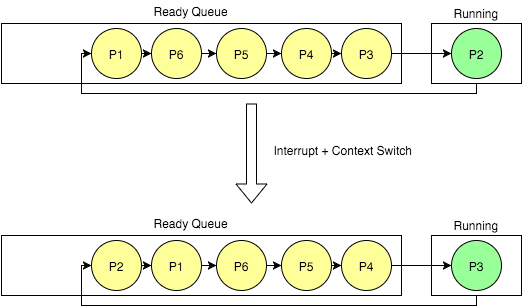
\includegraphics[width=0.8\textwidth]{includes/figures/chapter5_round_robidn_diagram.png}  \\
\caption{Implementation - Diagram of Round Robin without priority}
\end{center}
\label{fig:chapter5_round_robidn_diagram}
\end{figure}



Once the PCB has been chosen, the CPU state is switched to program mode, the register R1 to R12 pushed into the stack. Then the stack pointer and link pointer of the process that was running prior to the interruption is stopped is stored into its context, and the state in the PCB table is changed to \textit{READY}. Immediately after, the context are switched and the switched context is now ready to be run when the interrupts finishes.

Please find on figure \ref{fig:chapter5_snippet_context_switch} the relevant code snippet in charge of performing the context switch.

\begin{figure}[H]
\begin{minipage}{\linewidth}
\begin{lstlisting}[frame=single]
if (current_pcb != NULL) {
    __asm("cps #0x13"); // Switch to program mode in order to access the registers and stack pointer
    __asm("push {r0-r12}");
    __asm("mov %0, sp" : "=r" (current_pcb->context.sp));
    __asm("mov %0, lr" : "=r" (current_pcb->context.lr));
}

// Restore saved context
__asm("mov sp, %0" :: "r" (pcb_to_switch->context.sp));
__asm("mov lr, %0" :: "r" (pcb_to_switch->context.lr));
if (pcb_to_switch->state != NEW) {
    __asm("pop {r0-r12}");
}
\end{lstlisting}
\end{minipage}
\caption{Snippet presenting the context switch}
\label{fig:chapter5_snippet_context_switch}
\end{figure}

